
\chapter{ವರದಿ ನೀಡಿದ ಲ್ಯಾಂಬ್​ಟನ್​ ತಲೆಗೇ ಟ್ರಿಗನಮಿಟ್ರಿಕಲ್​ ಸರ್ವೇಯ ಭಾರ}

ಈ ಟ್ರಿಗನಮಿಟ್ರಿಕಲ್​ ಸರ್ವೇಯಲ್ಲಿ ತೊಡಗಿಸಿಕೊಂಡ ಮಹನೀಯರು ಯಾರೆಂದರೆ, ಮಿಲಿಟರಿ ಸೇವೆಗೆ ಬಂದು, ನಂತರ ತಮ್ಮ ಮ್ಯಾಪಿಂಗ್​ ಕಾರ್ಯದಲ್ಲಿನ ಬಲವಾದ ಹುಚ್ಚು, ಆಸಕ್ತಿ, ಪ್ರತಿಭೆ ಪಾಂಡಿತ್ಯದಿಂದ, ಸರ್ವೇಯಿಂಗ್​ನಂತಹ ನಾಗರೀಕ ಸೇವೆಗೆ ನೀಯೋಜಿತರಾದ ಮಿಲಿಟರಿ ಇಂಜಿನಿಯರುಗಳು. ಮಿಲಿಟರಿ ಕಾರ್ಯವಾದರೆ ಅಲ್ಲಿನ ಯುದ್ಧ ಕಾರ್ಯಾಚರಣೆಗೆ, ಸಾಕಷ್ಟು ಇನಾಮು ಪುರಸ್ಕಾರ ಇದ್ದೇ ಇರುತ್ತದೆ. ಯುದ್ಧ ಸೋತ ದೇಶದ ಸಕಲ ಸಿರಿ ಸಂಪತ್ತು ಮೊದಲಿಗೆ ಯುದ್ಧ ಗೆದ್ದ ಸೈನ್ಯದ ಸ್ವತ್ತು. ಆದರೆ, ಸರ್ವೇ ಕಾರ್ಯಕ್ಕೆ ನಿಯೋಜಿತರಾದರೆ, ಸಂಪೂರ್ಣ ಸಮರ್ಪಣಾ ಭಾವದಿಂದ ದುಡಿಯಬೇಕು. ಅದಕ್ಕೆ ಪ್ರತಿಯಾಗಿ ಹೇಳಿಕೊಳ್ಳುವ ಅಂತಹ ಬಹುಮಾನ ಇನಾಮು ಏನೂ ಇರುವುದಿಲ್ಲ. ಆದರೂ ಆ ಮಹನೀಯ ಸರ್ವೇಯರುಗಳು, ತಮ್ಮ ಸ್ವಯಂ ಸಾಮರ್ಥ್ಯದಿಂದ ಆಸಕ್ತಿಯಿಂದ ಮ್ಯಾಪಿಂಗ್​ ವಿಜ್ಞಾನದ ಸಾಧನೆಗಾಗಿ ದುಡಿದಿದ್ದಾರೆ. ಯುದ್ದ ಭೂಮಿಯಷ್ಟೇ ಭಯಾನಕ, ಸಾವು ನೋವಿನ ಪರಿಸ್ಥಿತಿಯಲ್ಲೂ, ಕಠಿಣ ಹವಮಾನದಲ್ಲೂ ಕಾರ್ಯ ನಿರ್ವಹಿಸಿದ್ದಾರೆ. ಗ್ರೇಟ್​ ಟ್ರಿಗನಮಿಟ್ರಿಕಲ್​ ಸರ್ವೇ ಯೋಜನೆಯ ಸಾವು ನೋವಿನ ಸಂಖ್ಯೆ ಯಾವುದೇ ಪ್ರಸಿದ್ದ ದೊಡ್ಡ ಯುದ್ದಕ್ಕಿಂತಲೂ ಹೆಚ್ಚು.

\enginline{1799}ರ ನವೆಂಬರ್​ನಲ್ಲಿ ಲ್ಯಾಂಬ್​ಟನ್​ರವರು ತಮ್ಮ ‘ಮೆರಿಡಿಯನಲ್​ ಆರ್ಕ್ ಮೆಜರ್\break ​ಮೆಂಟ್​ ಮತ್ತು ಟ್ರಿಗನಮಿಟ್ರಿಕಲ್​ ಸರ್ವೆ ಯೋಜನೆ’ಗಾಗಿ ವರದಿಯನ್ನು ಸಲ್ಲಿಸಿದ್ದರು. ಗಣಿತೀಯ ಹಾಗು ವೈಜ್ಞಾನಿಕ ಸರ್ವೇಗಾಗಿ ಲ್ಯಾಂಬ್​ಟನ್​ರವರು ಸಲ್ಲಿಸಿದ ಪ್ರಸ್ತಾವನೆಗೆ ಸರ್​ ಅರ್ಥರ್​ ವೆಲ್ಲಸ್ಲಿಯವರ ಸಮರ್ಥನೆ ಹಾಗೂ ಸಹಾಯ ಸಿಕ್ಕಿತು. ಹಾಗೂ ಮದ್ರಾಸ್​ ಸರ್ಕಾರದ ಅನುಮೋದನೆಯೂ ದೊರೆಯಿತು. ಈ ಅಳತೆ ಕಾರ್ಯಕ್ಕೆ ಲ್ಯಾಂಬ್​ಟನ್​ರವರನ್ನೇ ಮುಖ್ಯಸ್ಥರನ್ನಾಗಿ ನೇಮಿಸಲಾಯಿತು.

\begin{figure}[!htbp]
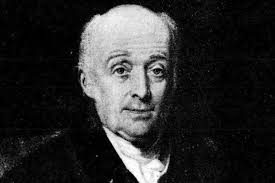
\includegraphics[scale=1.1]{"images/image005.jpg"}
\caption{ಕರ್ನಲ್​ ವಿಲಿಯಂ ಲ್ಯಾಂಬ್​ಟನ್​ರವರು}\label{chap4-fig1}
\end{figure}

ಲ್ಯಾಂಬ್​ಟನ್​ರವರಿಗೆ ಮ್ಯಾಥ್​ಮೆಟಿಕ್ಸ್​, ಮೆಕ್ಯಾನಿಕ್ಸ್​, ಅಸ್ಟ್ರನಮಿ ಇವು ಕರಗತ ವಿಷಯಗಳು. ಅವರಿಗೆ ಜಿಯೋಡೆಸಿಯಲ್ಲಿಯೂ ವಿಶೇಷ ಆಸಕ್ತಿ ಹಾಗೂ ಪರಿಣತಿ ಇತ್ತು. ಜಿಯೋಡೆಸಿ ಅಥವಾ ಭೂಗಣಿತ ಎಂದರೆ ಭೂಮಿಯ ಗಾತ್ರ, ಆಕಾರ ಇವುಗಳ ಅಧ್ಯಯನದ ವಿಷಯ. ಎಲ್ಲಾ ಪ್ರಮುಖ ವಿಜ್ಞಾನ ಪ್ರಕಟಣೆಗಳನ್ನೂ ಆಳವಾಗಿ ಓದಿ ಅವುಗಳನ್ನು ಅರಗಿಸಿಕೊಳ್ಳುವುದು ಲ್ಯಾಂಬ್​ಟನ್​ರವರ ಹವ್ಯಾಸ. ಬ್ರಿಟೀಷ್​ ಆರ್ಡನನ್ಸ್​ ಸರ್ವೇಯ ಸ್ಥಾಪಕ ವಿಲಿಯಮ್ ರಾಯ್​\break ಮತ್ತು ಅವರ ಪ್ರಾನ್ಸ್​ನ ಮೂಲ ಗುರುಗಳು ಇವರುಗಳ ಟ್ರಿಗನಮಿಟ್ರಿಕಲ್​ ಮತ್ತು ಆರ್ಕ್\break ಮೆಸರ್​ಮೆಂಟ್​ ಕಾರ್ಯದಲ್ಲಿಯೂ ಸಹ ಅಪಾರ ಆಸಕ್ತಿಯನ್ನು ಹೊಂದಿದ್ದರು.\break ಲ್ಯಾಂಬ್​ಟನ್​ರವರು ಕೆನಡಾದಲ್ಲಿದ್ದಾಗ ಮಾಡಿದ್ದ ಸರ್ವೇ ಕಾರ್ಯವು ಟ್ರೈಯಾಂಗ್ಯುಲೇಷನ್ನಿನ ಸರಳ ತತ್ವವನ್ನು ಆಧರಿಸಿತ್ತು. ಅವರು ಕೆನಡಾದಲ್ಲಿರುವಾಗ ಸೂರ್ಯ ಗ್ರಹಣವನ್ನು ಸುರಕ್ಷತೆಯ ಕ್ರಮ ಮರೆತು, ಟೆಲಿಸ್ಕೋಪ್​ ಮೂಲಕ, ಬರಿಗಣ್ಣಲ್ಲಿ ನೋಡಿಬಿಟ್ಟಿದ್ದರು. ಇದರಿಂದ ಅವರ ಎಡಗಣ್ಣು ಗಾಜುಗಣ್ಣು ಆಗಿ ಭಾಗಶಃ ಶಕ್ತಿ ಕಳೆದುಕೊಂಡಿತ್ತು.

ನಾಲ್ಕನೇ ಮೈಸೂರು ಯುದ್ಧದಲ್ಲಿ ಟಿಪ್ಪು ವಿರುದ್ಧ ಹೋರಾಡಿದ ಸೈನ್ಯದಲ್ಲಿ ಇನ್​ಫ್ಯಾಂಟ್ರಿ ಆಫೀಸರ್​ ಆಗಿದ್ದವರು ಕರ್ನಲ್​ ವಿಲಿಯಂ ಲ್ಯಾಂಬ್​ಟನ್​ರವರು. ಇವರ ಜನನ \enginline{1753}. ಲ್ಯಾಂಬ್​ಟನ್​ರವರು ಇಂಗ್ಲೆಂಡಿನ ತಮ್ಮ ಊರು, ಕುಟುಂಬ ಮತ್ತು ತಂದೆ ತಾಯಿಯ ವಿಚಾರವಾಗಿ, ಯಾರೊಂದಿಗೂ ಅಷ್ಟಾಗಿ ಹಂಚಿಕೊಳ್ಳುತ್ತಿರಲಿಲ್ಲ. ಈ ವಿಚಾರದಲ್ಲಿ ಅವರದ್ದು ಬಹಳ ಸಂಯಮ ಮತ್ತು ಬಿಗುವಿನ ನಡತೆ. ಆದ್ದರಿಂದ ಅವರು ಇಂಗ್ಲೆಂಡ್​ನಲ್ಲಿ ಎಲ್ಲಿ ಜನಿಸಿದರು ಮತ್ತು ತಂದೆ ತಾಯಿ ಯಾರು ಎಂದು ಸರಿಯಾಗಿ ತಿಳಿದಿಲ್ಲ.

ಲ್ಯಾಂಬ್​ಟನ್​ರವರನ್ನೇ ಅವರ ಪ್ರಸ್ತಾವನೆಯ ಟ್ರಿಗನಮಿಟ್ರಿಕಲ್​ ಸರ್ವೇ ಕಾರ್ಯಕ್ಕೆ ನೇಮಿಸಿದ್ದರಿಂದ, ಈ ಕಾರ್ಯದ ಯಶಸ್ಸಿಗೆ ಅವಶ್ಯವಾದ ಸಮರ್ಥ ಸಿಬ್ಬಂದಿಯನ್ನು ಅವರು ಸಂಘಟಿಸಿಕೊಳ್ಳತೊಡಗಿದರು. ಲೆಫ್ಟಿನೆಂಟ್​ ವಾರೆನ್​ ಮತ್ತು ಲೆಫ್ಟಿನೆಂಟ್​ ಕೇಟರ್​ರಂತಹ ಸಮರ್ಥ ಪ್ರತಿಭಾವಂತರನ್ನು ಸಹಾಯಕರನ್ನಾಗಿ ನೇಮಿಸಿಕೊಂಡರು. ಸಮರ್ಥ ಸಿಬ್ಬಂದಿಯ ಜೊತೆಗೆ ಅವಶ್ಯವಾದ ಸೂಕ್ತ ಉಪಕರಣಗಳನ್ನು ವ್ಯವಸ್ಥೆ ಮಾಡಿಕೊಳ್ಳಬೇಕಾಯಿತು. ಅವರ ಕಾಲದ ಪದ್ಧತಿಯೆಂದರೆ, ಅಧಿಕಾರಿಗಳೇ ತಮ್ಮ ಸರ್ವೇ ಕಾರ್ಯಕ್ಕೆ ಅಗತ್ಯವಿರುವ ಉಪಕರಣಗಳನ್ನು ಸರಬರಾಜು ಮಾಡಿಕೊಳ್ಳಬೇಕಿತ್ತು. ಜೆನಿತ್​ ಸೆಕ್ಟರ್​ ಮತ್ತು ಸ್ಟೀಲ್​ ಚೈನನ್ನು ಕೋಲ್ಕತ್ತಾದಿಂದ ತರಿಸಿಕೊಳ್ಳಲಾಯಿತು.

ಜೆನಿತ್​ ಸೆಕ್ಟರ್​ ಉಪಕರಣವು ಖಗೋಳ ವೀಕ್ಷಣೆಗೆ ಬಳಸುವ ಮೂಲ ಉಪಕರಣ. ಜೆನಿತ್​ ಮತ್ತು ನಕ್ಷತ್ರಗಳ ನಡುವಿನ ಕೋನವನ್ನು ಅಳೆಯಲು ಇದನ್ನು ಉಪಯೋಗಿಸಲಾಗುತ್ತದೆ. ಇದು ಮುಖ್ಯವಾಗಿ ಟೆಲಿಸ್ಕೋಪ್​ ಮತ್ತು ಲಂಬ ಸಮತಲದಲ್ಲಿನ ಕೋನಮಾಪಕಗಳನ್ನು ಹೊಂದಿದೆ. ಲಂಬ ಸಮತಲದಲ್ಲಿನ ಕೋನಮಾಪಕವು ತ್ರಿಜ್ಯ ಖಂಡವಾಗಿದೆ. ಅಂದರೆ, ಸರ್ಕಲ್​ನ ಸೆಕ್ಟರ್​ ಆಗಿದೆ. ಟೆಲಿಸ್ಕೋಪ್​ ಮೂಲಕ ನಕ್ಷತ್ರ ವೀಕ್ಷಣೆ ಮಾಡಿ, ಅವುಗಳ ಸ್ಥಾನಗಳನ್ನು ಗ್ರಾಜ್ಯುಯೇಟೆಡ್​ ಸೆಕ್ಟರ್​ ಮೇಲೆ ಡಿಗ್ರಿ ಮಿನಿಟ್​ ಸೆಕೆಂಡ್​ಗಳಲ್ಲಿ ನಿಖರವಾಗಿ ಓದಲಾಗುತ್ತದೆ. ಇದರಿಂದ ವೀಕ್ಷಣಾ ತಾಣದ ಅಕ್ಷಾಂಶ ಮತ್ತು ರೇಖಾಂಶಗಳನ್ನು ಲೆಕ್ಕಾಚಾರ ಮಾಡಬಹುದು. ಸ್ಟೀಲ್​ ಚೈನು ಟ್ರಿಗನಮಿಟ್ರಿಕಲ್​ ಸರ್ವೇಯಲ್ಲಿ ಬೇಸ್​ಲೈನಿನ ಅಳತೆಗೆ ಬಳಸುವ ಉಪಕರಣ. ಈ ಸ್ಟೀಲ್​ ಚೈನು ನೂರು ಅಡಿ ಉದ್ದವಿದ್ದು, ಪ್ರತಿ ಲಿಂಕು \enginline{2.5} ಅಡಿ ಇರುವ, \enginline{40} ಲಿಂಕುಗಳಿಂದ ಕೂಡಿತ್ತು. ಈ ಚೈನಿನ ತೂಕವು ಸುಮಾರು \enginline{50} ಕೆ.ಜಿ. ಅದರ ಚಾರಿತ್ರಿಕ ಪ್ರಾಮುಖ್ಯತೆಗಾಗಿ ಈಗಲೂ ಡೆಹರಾಡೂನಿನಲ್ಲಿ ಇದನ್ನು ಸುರಕ್ಷಿತವಾಗಿ ಇಡಲಾಗಿದೆ.

\begin{figure}[!htbp]
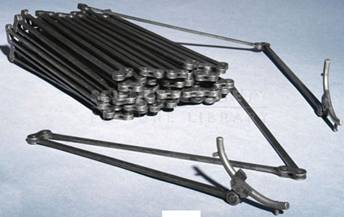
\includegraphics[scale=1.15]{"images/image006.jpg"}
\caption{ಬೇಸ್‌ಲೈನ್ ಅಳತೆಗೆ ಸರಪಳಿ}\label{chap4-fig2}
\end{figure}

